\section{The Agent}

\subsection{Create Customer Profile}
\textbf{Pre-conditions}: The Agent must be able to help a customer
to make a profile.

\textbf{Post-conditions}: Customer successfully created a profile.

\textbf{Purpose}: The Agent be able to know which customer prefer
what show.

\textbf{Description}: The Agent be able to check on if the customer
has successfully made a profile and if their profile is correct or
not.

\subsection{Buy tickets}
\textbf{Pre-conditions}: The Agent must be able to know how many
tickets are available and how many ticket have been sold altogether.

\textbf{Post-conditions}: The Agent successfully sold the tickets.

\textbf{Purpose}: The Agent need to keep track with the amount of
tickets that that customer are buying.

\textbf{Description}: The Agent always has to check on the system
and keep track on how the tickets are selling and how many tickets
are available.

\subsection{Update Customer Profiles}
\textbf{Pre-conditions}: The Agent need to verify whether the
customer has made changes to their profile.

\textbf{Post-conditions}: The Agent successfgully verified the
customer changes to their profile.

\textbf{Purpose}: The purpose for this is that if a customer makes
changes to their customer profile the Agent be able to verify it.

\textbf{Description}: The Agent need to always check whether the
customer made changes to their profile if theire is a changes the
Agent would not know if their profile is correct or not.

\subsection{See Sold Tickets}
\textbf{Pre-conditions}: The Agent must checkhow many tickets are
sold for the show.

\textbf{Post-conditions}: The Agent successfully checked the amount
of ticket sold to each show.

\textbf{Purpose}: The purpose for this is that the Agent need to
always keep track with the amount of tickets sold to each show.

\textbf{Description}: The Agent have to check if the tickets are
being sold or not and how many tickets are being sold to each
customer.

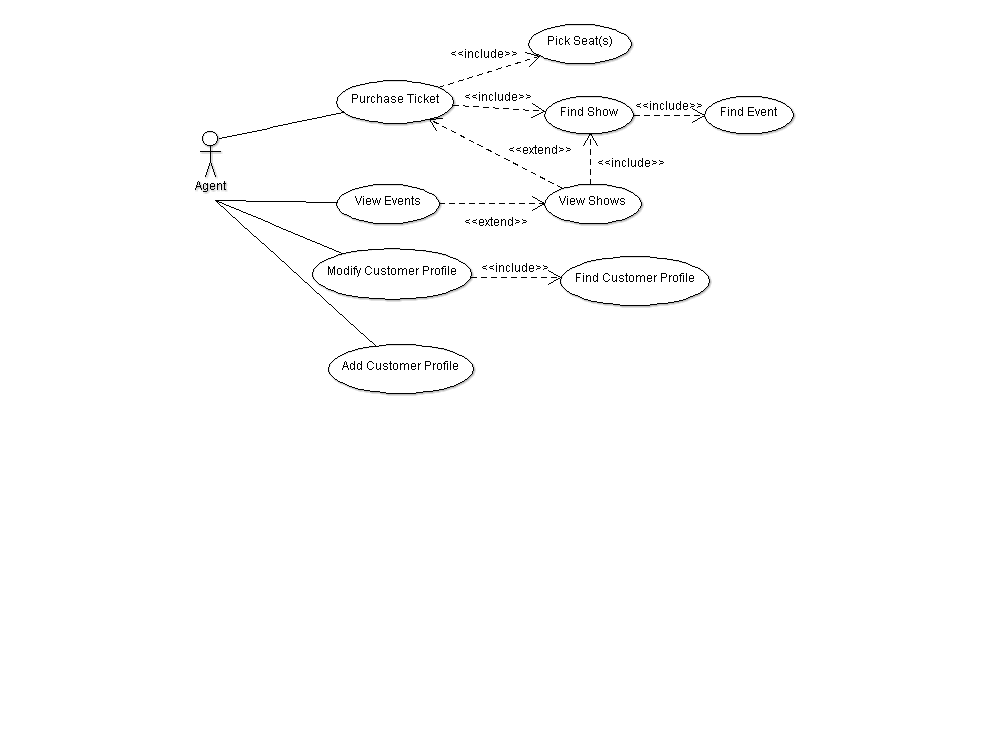
\includegraphics[width=\linewidth]{AgentUsecaseDiagram}
